\section{Inroduction}

\textbf{Error detection}

Regardless of the design of the transmission system, there will be errors, resulting
in the change of one or more bits in a transmitted frame. In what follows, we assume that data are transmitted as one or more contiguous sequences of bits,
called frames. 
the probability that a frame arrives with no bit
errors decreases with increasing frame length; the longer the frame, the more bits it
has and the higher the probability that one of these is in error. This is the kind of result that motivates the use of error-detecting techniques.All
of these techniques operate on the following principle  For a given frame
of bits, additional bits that constitute an \emph{error-detecting code} are added by the transmitter.

\begin{figure}[!htbp]
	\centering
	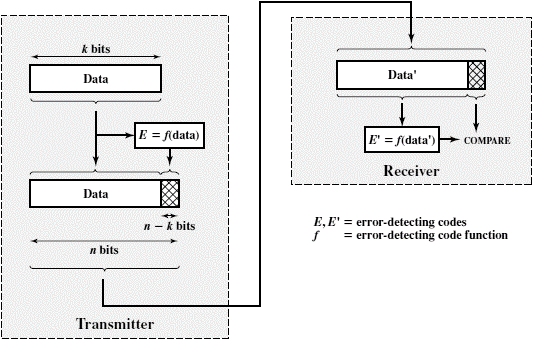
\includegraphics [scale=0.55]{images/Intro/Imagen1.png}
	\caption{Error Detection Process}
\end{figure}



\textbf{Cyclic Redundancy Check (CRC)}\\

One of the most common, and one of the most powerful, error-detecting codes is the
cyclic redundancy check (CRC), which can be described as follows. Given a k-bit
block of bits, or message, the transmitter generates an sequence, known
as a frame check sequence (FCS), such that the resulting frame, consisting of n bits,
is exactly divisible by some predetermined number. The receiver then divides the
incoming frame by that number and, if there is no remainder, assumes there was no
error.3
To clarify this, we present the procedure in three equivalent ways:

\begin{itemize}
	\item Modulo 2 arithmetic
	\item Polynomials
	\item Digital logic
\end{itemize}

The methods seen in class where the first two.\\


\textbf{Modulo 2 arithmetic}\\

Modulo 2 arithmetic uses binary addition with no carries,
which is just the \textbf{ exclusive-OR (XOR)} operation. Binary subtraction with no carries
is also interpreted as the XOR operation.

Now define

\begin{equation*}
	T = 2n-kD + F
\end{equation*}

Where: \\
$P =$ pattern of $n - k + 1$ bits; this is the predetermined divisor\\
$F = (n - k)$-bit FCS, the last $(n - k) $bits of $T$\\
$D =$ $k-$bit block of data, or message, the first $k $bits of $T$\\
$T$= $n$-bit frame to be transmitted \\

According with Tebauhman:\\

CRC (Cyclic Redundancy Check is  also known
as a \textbf{polynomial code}. Polynomial codes are based upon treating bit strings as
representations of polynomials with coefficients of 0 and 1 only. A k-bit frame is
regarded as the coefficient list for a polynomial with $k-$terms, ranging from $x^{k-1}$
to $x^0$.

For example, 110001 has 6 bits and thus represents a six-term polynomial with
coefficients 1, 1, 0, 0, 0, and $ 1: 1x^5 + 1x^4 + 0x^3 + 0x^2 + 0x^1 + 1x^0.$

When the polynomial code method is employed, the sender and receiver must
agree upon a \textbf{ generator polynomial, $\mathbf{G(x)}$}, in advance.  To compute the CRC for some frame with
m bits corresponding to the polynomial $ \mathbf{M(x)}$, the frame must be longer than the
generator polynomial.  When the receiver gets the checksummed frame, it tries dividing it
by G(x). If there is a remainder, there has been a transmission error.

\begin{figure}[!htbp]
	\centering
	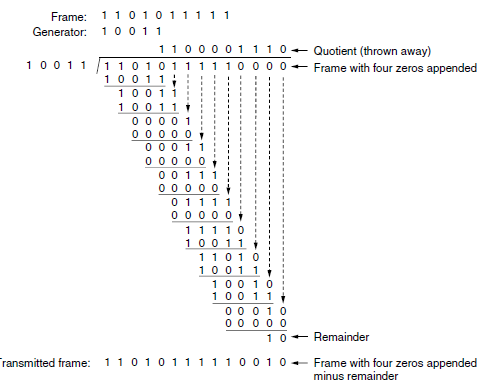
\includegraphics [scale=0.55]{images/Intro/Imagen2.png}
	\caption{Error Detection Process}
\end{figure} 